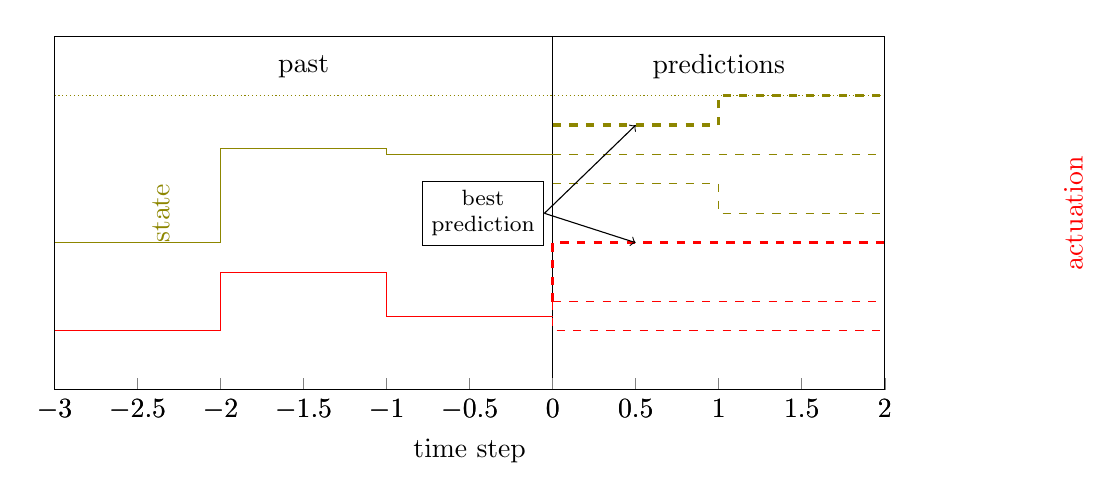
\begin{tikzpicture}

\begin{axis}[
        at={(0, 0)},
        xlabel=time step,
        ylabel={\color{olive}state},
        ytick pos = left,
        xtick pos = bottom,
        xmin = -3,
        xmax = 2,
        ymin = 0,
        ymax = .6,
        yticklabel=\empty,
        ytick style={draw=none},
        y label style={at={(axis description cs:0.15,.5)},anchor=south},
width = \linewidth, 
height = .5\linewidth
]

\addplot[densely dotted, olive] coordinates{
(-3, .5)
(2, .5)
};
\addplot[no marks, black] coordinates{
(0, 0)
(0, .6)
};

\addplot[ olive] coordinates{
(-3, .25)
(-2, .25)
(-2, .41)
(-1, .41)
(-1, .4)
(-0, .4)
(0, .4)
};
\addplot[dashed, olive, very thick] coordinates{
(0, .45)
(1, .45)
(1, .5)
(2, .5)
};
\addplot[dashed, olive] coordinates{
(0, .4)
(1, .4)
(1, .4)
(2, .4)
(2, .45)
};
\addplot[dashed, olive] coordinates{
(0, .35)
(1, .35)
(1, .3)
(2, .3)
};

\draw[->, align=center] (axis cs: -.05,.3) node[left, font=\footnotesize, rectangle, draw] {best\\prediction} -- (axis cs: .5, .45);

\end{axis}

\begin{axis}[
        at={(0, 0)},
        ylabel={\color{red}actuation},
        ytick pos = right,
        xtick pos = bottom,
        xmin = -3,
        xmax = 2,
        ymin = 0,
        ymax = 6,
        yticklabel=\empty,
        ytick style={draw=none},
        y label style={at={(axis description cs:1.25,.5)},anchor=south},
width = \linewidth, 
height = .5\linewidth
]

\addplot[red] coordinates{
(-3, 1)
(-2, 1)
(-2, 2)
(-1, 2)
(-1, 1.25)
(0, 1.25)
};

\addplot[red, dashed, very thick] coordinates{
(0, 1.5)
(0, 2.5)
(2, 2.5)
};

\addplot[red, dashed] coordinates{
(0, 1.5)
(0, 1.)
(2, 1.)
};

\addplot[red, dashed] coordinates{
(0, 1.5)
(0, 1.5)
(2, 1.5)
};

\draw[->, align=center] (axis cs: -.05,3.) -- (axis cs: .5, 2.5);

\node at (axis cs: -1.5, 5.5) {past};
\node at (axis cs: 1, 5.5) {predictions};

\end{axis}

\end{tikzpicture}